\documentclass[11pt]{article}
\usepackage[a4paper,margin=1in]{geometry}
\usepackage{amsmath,amssymb,graphicx,booktabs,array,longtable,microtype,hyperref,float,pdflscape,enumitem}
\usepackage[T1]{fontenc}
\usepackage{lmodern}
\hypersetup{colorlinks=true,linkcolor=blue,citecolor=blue,urlcolor=blue}
\newcommand{\Vcal}{\mathcal{V}}
\begin{document}

\title{Supplementary Information for\\From Trace to Modal Closure: Dynamic Conditions for Regenerative Reentry in a Path-Dependent Adaptive System}
\author{Gregorio Rozas Fern\'andez \\ Independent Researcher}
\date{October 4, 2026}
\maketitle

\section{Supplementary methods}

\subsection{Evidence hierarchy and prospective design freezing}

Paper IV followed a diagnostic-to-confirmatory workflow. Diagnostic experiments were used to refine hypotheses, identify observables, or falsify candidate mechanisms. Confirmatory designs were subsequently frozen in the internal research record before fresh seed cohorts were executed. Because this freezing was not independently timestamped in an external registry, the paper uses the phrase \emph{prospectively frozen confirmatory criteria} rather than external preregistration.

Most central confirmatory experiments used 64 fresh seeds. Important exceptions include the 32-instance common-map diagnostic and the independent 16-seed native-autocorrection replication. Inference was experiment specific and used combinations of nonparametric 95\% bootstrap intervals, favorable-seed or favorable-cell fractions, one-sided sign-flip/randomization tests, Holm correction for specified hypothesis families, and frozen effect-size thresholds. Final transcript-coded analyses frequently used 150,000 bootstrap resamples, but this number is not retroactively assigned to earlier experiments where the exact analysis implementation was not independently archived. No single global multiplicity correction was imposed across the full longitudinal sequence of distinct experiments; multiplicity control was applied within the hypothesis families specified by each frozen design. The separation of fresh confirmatory cohorts from diagnostic/exploratory blocks and the complete evidence audit are therefore part of the inferential record.

\subsection{Full reactor constants and dimensions}

\begin{table}[H]
\caption{Core reactor dimensions and constants used in Paper IV.}
\begin{tabular}{lll}
Quantity & Value / shape & Construction\\
\hline
Recurrent state $x$ & $32$ & 4 modules $\times$ 8 units\\
Body/environment/action & $4$ each & $s,e,a\in\mathbb{R}^4$\\
Context $c$ & $8$ & $c=S_ee+S_aa+\eta_c$\\
Slow memory $m$ & $8$ & decay $0.98$, write rate $0.02$\\
Plastic state $\theta$ & $4$ & clipped to $[-0.25,0.25]$\\
Relevance $r$ & $12$ & decay $0.98$, rate $0.02$\\
Boundary trace $K$ & $8\times4$ & decay $0.98$, rate $0.02$\\
History $g_h$ & up to 5 $\times$ 4 & exponentially weighted module means\\
$W_0$ sparsity & $p_{\rm in}=0.35$, $p_{\rm out}=0.05$ & nonzero $\mathcal N(0,0.35)$\\
$\rho(W_0)$ & $0.75$ & spectral normalization\\
$B_{\rm in}$ & $32\times12$ & $\mathcal N(0,0.18)$\\
$M$ & $32\times8$ & $\mathcal N(0,0.12)$\\
$P_m$ & $8\times32$ & $\mathcal N(0,1/\sqrt{32})$\\
$S_e$ & $8\times4$ & $\mathcal N(0,0.18)$\\
$S_a$ & $8\times4$ & 4 nonzero rows, $\mathcal N(0,0.30)$\\
$J_p,J_r,J_b$ & $32\times4,32\times12,32\times8$ & SD $0.04,0.025,0.025$\\
Recurrent leak & $0.25$ nonlinear update & $x_{t+1}=0.75x_t+0.25\tanh z_t$\\
Body noise SD & $0.005$ & matched where required\\
Context noise SD & $0.02$ & matched where required\\
Action exploration SD & $0.02$ & matched where required\\
Finite-difference $\epsilon$ & $10^{-4}$ & operator experiments\\
Write / return windows & 24 / 24 steps & isolated relay experiments\\
\end{tabular}
\end{table}

The full recurrent update is given in the main Methods. For completeness, the adaptive updates that are easiest to lose when the model is described only verbally are
\begin{align}
 e_{t+1}&=0.95e_t+0.03\eta^{\mathrm{env}}_t+\mu_t,\\
 r_{t+1}&=0.98r_t+0.02u_{t-1}\Delta\Vcal_t,\\
 m_{t+1}&=0.98m_t+0.02P_mx_{t+1},\\
 K_{t+1}&=0.98K_t+0.02c_t\zeta_{t-1}^{T},\\
 \theta_{t+1}&=\operatorname{clip}\!\left[\theta_t+0.002(\chi^*-\chi_{t+1})-0.004\theta_t+0.0005\Delta\Vcal_t p^{\mathrm{post}}_t,-0.25,0.25\right],
\end{align}
where $\Delta\Vcal_t$ is computed from the pre-action viability at the beginning of the step, $\chi_{t+1}$ is the vector of module-wise mean squared activities after the recurrent update, and $p^{\mathrm{post}}_t$ includes the newly appended module-mean vector. The recurrent drive instead uses $p^{\mathrm{pre}}_t$, computed from the history deque before appending the current module means.

\paragraph{Exact C4 within-step order.}
The recovered base source updates a timestep in the following order. This order is part of the model specification rather than an implementation convenience.
\begin{enumerate}[leftmargin=1.6em,itemsep=1pt,topsep=2pt]
\item Update the environmental state $e$ and apply any protocol-defined body kick.
\item Compute current context $c=S_ee+S_aa+\eta_c$, concatenate $u=[s;c]$, evaluate pre-action viability, and form $\Delta\Vcal$ relative to the stored previous viability.
\item Update relevance $r$ from the previous input $u_{t-1}$ and $\Delta\Vcal$.
\item Form the relevance-modulated effective input $u_{\mathrm{eff}}$, construct $W(\theta)$, and initialize the recurrent drive.
\item Update $K$ from current context and previous action noise; compute the row-norm scores, collective median, and $b$.
\item Compute $p^{\mathrm{pre}}$ from the existing history deque and add the $J_p p+J_r r+J_b b$ recurrent drives.
\item Update recurrent state $x$ and apply any protocol-defined lesion/reset.
\item Compute current module means $g$ and append $g$ to the five-entry history deque.
\item Update the action from the new $x$-derived $g$, current body state, and current action noise.
\item Update body state $s$; Paper-IV relation histories use $R_4(\phi)$ in the action-to-body term.
\item Update slow memory $m$ from the new recurrent state.
\item Recompute $p^{\mathrm{post}}$ from the updated history deque and update $\theta$.
\item Store current $u$, action noise, and the pre-action viability as the lagged quantities for the next step.
\end{enumerate}
The reference reconstruction of the relational branch uses the same standard counter-clockwise planar rotation in coordinates $(1,2)$ and $(3,4)$ and is independently checked by the recovered causal-angle estimator.

\paragraph{Metric definitions.}
For nonzero vectors $a,b$, sign-invariant directional similarity and angle are
\begin{equation}
 c_{\pm}(a,b)=\frac{|a^Tb|}{\|a\|\|b\|},\qquad \alpha_{\pm}(a,b)=\arccos c_{\pm}(a,b).
\end{equation}
For unit vectors $v,w$, one-dimensional subspace displacement is $d_P(v,w)=\|vv^T-ww^T\|_F$. The half-channel interface efficiency is
\begin{equation}
 \eta_{\mathrm{int}}=\frac{\sigma_1(BA)}{\sigma_1(A)\sigma_1(B)},
\end{equation}
and normalized non-normality is
\begin{equation}
 \nu(T)=\frac{\|T^TT-TT^T\|_F}{\|T\|_F^2}.
\end{equation}
Representational-similarity analysis (RSA) compares vectorized pairwise dissimilarity structures under the correlation rule frozen for that experiment. In T01, the empirical structure consists of pairwise standardized future-response distances and the target structure consists of true circular chord distances between donor relations. T06 analogously compares relative history--present angular geometry. Where the recovered design records only ``correlation'' rather than the exact correlation-family implementation, the release does not retroactively relabel it Pearson or Spearman. Shuffle advantages are the observed RSA minus the mean RSA under the corresponding frozen label or component shuffle.

For C07, the observed test-context closure need is
\begin{equation}
 n_{\mathrm{actual}}=1-|u_B^Tv_B|,
\end{equation}
while the dynamic prediction from the calibration map is
\begin{equation}
 n_{\mathrm{pred}}=1-|u_B^T C_{\mathrm{dyn}}^{A}u_B|,
\end{equation}
with unit-normalized modal vectors; closure-need error is $|n_{\mathrm{pred}}-n_{\mathrm{actual}}|$. Multigenerational relative amplitude, modal alignment, and compatible share are $a_g=\|d_g\|/\|d_0\|$, $F_g=c_{\pm}(d_g,v)$, and $S_g=F_g^2$.

\paragraph{Carrier nomenclature.}
The archived R06/R07/C03/C07 code and CSV schemas use historical labels \texttt{G0} and \texttt{G1} for two operator carriers. To avoid collision with generation labels G1--G4, the manuscript calls these $q_{\mathrm{cal}}$ (calibration carrier) and $q_{\mathrm{test}}$ (test carrier). Archival filenames, JSON fields, and CSV column names are not rewritten.

\subsection{Global evidence and inference audit}

Table~\ref{tab:global-audit} exposes every experiment retained in the main paper or Supplement. The compact criterion column summarizes the frozen primary decision rules; the release also includes \texttt{provenance/EVIDENCE\_AUDIT.csv}, which preserves the complete recovered H1--H4 strings from each available design JSON. Diagnostic and exploratory rows are not promoted to confirmatory status.

\begin{landscape}
\tiny
\setlength\LTleft{0pt}\setlength\LTright{0pt}
\renewcommand{\arraystretch}{1.12}
\begin{longtable}{p{0.65cm}p{2.25cm}p{2.55cm}p{3.15cm}p{3.9cm}p{6.1cm}p{2.2cm}}
\caption{Global audit of evidence status, design provenance, primary targets, frozen criteria, and outcomes.}\label{tab:global-audit}\\
\toprule
ID & Status & Cohort & Design provenance & Primary estimand & Frozen primary criterion(s), compact form & Outcome\\
\midrule
\endfirsthead
\toprule
ID & Status & Cohort & Design provenance & Primary estimand & Frozen primary criterion(s), compact form & Outcome\\
\midrule
\endhead
T01 & confirmatory pass & 73000--73063 (n=64) & original frozen JSON & response norm; response RSA & norm $>0.08$; RSA shuffle advantages $>0$; mean RSA $>0.07$ & PASS \\
T04 & confirmatory fail/null & 97000--97063 (n=64) & original frozen JSON & same-encounter gain / specificity & four signed predictions ($<0,<0,>0,>0$), each Holm/sign-flip + robustness & FAIL / null \\
T05 & confirmatory pass & 99000--99063 (n=64) & original frozen JSON & component norm and RSA & intact norm $>0.03$; $r$ ratio $>5$; K RSA $>0.65$; NO\_R--intact RSA $>0.45$ & PASS \\
T06 & confirmatory pass & 101000--101063 (n=64) & original frozen JSON & interaction fraction; K/M relative RSA & interaction $>0.50$; $r$ ratio $>100$; K/M RSA shuffle advantages $>0$ with raw floors & PASS \\
T07 & confirmatory pass & 103000--103063 (n=64) & original frozen JSON & correct two-trace span $R^2$ & pair-span $R^2>0.90$; correct--wrong $>0.25$; pair--single $>0.08$; older fraction $>0.30$ & PASS \\
F01 & confirmatory pass & 107000--107063 (n=64) & original frozen JSON & storage error vs readout nonadditivity & storage error $<0.02$; response error $<0.03$; readout excess $>0.05$; mismatch $<0.02$ & PASS \\
F02 & confirmatory pass & 110000--110063 (n=64) & original frozen JSON & stagewise residual; additive-$b$ collapse & row-norm residual $>0.04$; centering gain $>0.02$; sigmoid increment tiny; additive-$b$ action residual $<10^{-4}$ & PASS \\
F03 & confirmatory pass & 113000--113063 (n=64) & original frozen JSON & third-trace contextual interaction & normalized $b$ and action interactions $>0.10$; additive-$b$ removes $>0.999$ / $>0.99$ & PASS \\
F04 & confirmatory pass & 115000--115063 (n=64) & original frozen JSON & jump/path fraction; event curvature & max jump/path $<0.10$; rank and median curvature advantages $>0$; median $>$ generic rank & PASS \\
R01 & confirmatory pass & 121000--121063 (n=64) & original frozen JSON & cycle--flat response distance & cycle--flat response $>0.015$; $r>0.010$; $m>0.060$; return mismatch $>0.020$ & PASS \\
R02 & confirmatory pass & 123000--123063 (n=64) & frozen working record; JSON unavailable & removed-response fractions & frozen ablation decomposition; exact standalone criterion file unavailable & PASS \\
R03 & confirmatory pass & 127000--127063 (n=64) & original frozen JSON & $x\to m$ and $m\to x$ relay & relay contrasts $>0.25,0.20,0.15,0.15$ with favorable-seed/bootstrap rules & PASS \\
R04 & confirmatory pass & 147000--147063 (n=64) & original frozen JSON & write/return alignment gains & return rescue $>0.005$; specific rescue $>0.005$; write cosine $>0.15$; full return $>0.003$ & PASS \\
R05 & confirmatory pass & 149000--149063 (n=64) & original frozen JSON & projection rescue; G3 norm/cosine & G1 rescue $>0.08$; G2 $>0.015$; G3 norm $<0.015$; G3 cosine $>0.55$ & PASS \\
R06 & confirmatory pass & 151000--151063 (n=64) & original frozen JSON & $\sigma_1(T)$; finite top-mode gain & mean $\sigma_1(T)<0.15$; finite top gain $<0.15$; optimal--historical gain $>0.04$ & PASS \\
R07 & confirmatory pass & 153000--153063 (n=64) & original frozen JSON & $\sigma_1(A),\sigma_1(B)$; interface efficiency & $\sigma_1(A)<0.15$; $\sigma_1(B)/\sigma_1(A)>5$; ideal product $<0.20$; efficiency $<0.75$ & PASS \\
M01 & confirmatory pass & 157000--157063 (n=64) & original frozen JSON & inherited vs reoriented gain & capacity change $<10\%$; G2 inherited alignment $<0.40$; reoriented gain $>0.85$; G4 reoriented $>0.70$ & PASS \\
M02 & confirmatory pass & 159000--159063 (n=64) & original frozen JSON & mode cosine/angle/projector drift & consecutive $|\cos|>0.995$; angle $<2^\circ$; projector $<0.05$; relative $\sigma_1$ change $<0.05$ & PASS \\
M03 & confirmatory pass & 161000--161063 (n=64) & original frozen JSON & mode spread across histories & mean angle $<1.5^\circ$; max angle $<3^\circ$; $\sigma_1$ spread $<0.05$; projector $<0.04$ & PASS \\
M04 & confirmatory pass & 163000--163063 (n=64) & original frozen JSON & alignment$^2$ vs $\|\Delta m\|$ & Spearman $>0.85$; aligned/orthogonal imprint ratio $>2$; positive contrast in $>95\%$ seeds & PASS \\
M05 & confirmatory pass & 165000--165063 (n=64) & original frozen JSON & native/AMP/DIR compatibility & native $\rho>0.90$; AMP/DIR $\rho>0.85$; positive aligned contrasts in $>95\%$ seeds & PASS \\
M06 & confirmatory pass & 168000--168063 (n=64) & original frozen JSON & operator-predicted imprint & norm correlation and vector cosine $>0.995$; relative error $<0.005$; shuffle advantages $>0.70$ & PASS \\
M07 & diagnostic replication null & 166100--166115 (n=16) & independent diagnostic record & native autocorrection effects & diagnostic replication only; no confirmatory threshold & diagnostic null \\
M08 & confirmatory pass & 170000--170063 (n=64) & original frozen JSON & compatible share in $m$ and $x$ & memory share $>0.75$; returned share $>0.82$; return increment $>0.04$; residual sanity $<0.005$ & PASS \\
M09 & confirmatory pass & 172000--172063 (n=64) & original frozen JSON & $|u_1^Tv_1|$; non-normality & $|u_1^Tv_1|<0.50$; output--$u_1$ cosine $>0.995$; preference $>0.40$; $\sigma_1/\rho>1.5$ & PASS \\
C01 & confirmatory equivalence/null & 174000--174063 (n=64) & original frozen JSON & next-loop gain after co-product restoration & absolute gain differences $<0.002$; ALL\_NONX ratio in $[0.98,1.02]$ & NULL / equivalence \\
C02 & diagnostic null & 175000--175031 (n=32) & diagnostic working record & held-out common-map alignment & diagnostic held-out comparison; no frozen confirmatory threshold & diagnostic null \\
C03 & confirmatory pass & 176000--176063 (n=64) & original frozen JSON & own-instance transferred alignment & own $|\cos|>0.97$; own--identity and own--wrong $>0.50$; pair geometry $>0.98$ & PASS \\
C04 & confirmatory mixed/fail & 180000--180063 (n=64) & transcript-recovered design & reciprocity-specific closure gains & reciprocal advantage over matched controls $>0.05/0.04/0.025$; vs native $>0.04$ & mixed; strong H fail \\
C05 & confirmatory fail/null & 182000--182063 (n=64) & transcript-recovered design & subspace/basis closure gains & XSPACE gain $>0.08$; memory-only weak; interaction $>0.08$; BOTH alignment $>0.55$ & FAIL / heterogeneous \\
C06 & exploratory null & same 182000--182063 cohort (n=64 reused) & transcript-recovered design & static moderators; CV $R^2$ & post-confirmatory exploratory moderator predictions; no confirmatory threshold & exploratory null \\
C07 & confirmatory pass & 184000--184063 (n=64) & original frozen JSON & dynamic alignment; closure-need MAE & dynamic $|\cos|>0.995$; vs static $>0.20$; vs wrong $>0.70$; need MAE $<0.02$ & PASS \\
G01 & confirmatory pass & 186000--186063 (n=64) & original frozen JSON & G4 amplitude; specificity; alignment & G4 $>0.85$; vs unclosed $>0.70$; specificity $>0.60$; mean G1--G4 alignment $>0.99$ & PASS \\
G02 & confirmatory pass & 188000--188063 (n=64) & original frozen JSON & G4 share; $67.5^\circ/90^\circ$ boundary & nonorthogonal G4 share $>0.95$; $67.5^\circ$ gain $>0.70$; vs unclosed $>0.65$; G1 $90^\circ<0.10$ & PASS \\
\bottomrule
\end{longtable}
\end{landscape}

Inference was experiment specific. Confirmatory rows used the released frozen H1--H4 rules, generally combining effect-size thresholds, favorable-seed or favorable-cell fractions, bootstrap intervals, and, where specified in the design artifact, one-sided sign-flip/randomization tests with Holm correction. The exact design files and the exhaustive machine-readable audit should be treated as authoritative when a compact table entry omits a secondary threshold.

\subsection{Trace-weight continuation}

The main paper identifies median-relative collective readout as the principal source of nonadditivity in the $K$ branch. F04 varied trace weights continuously while following $b$ and downstream action. Generic rank-order events were distinguished from events in which a row crossed the collective median reference. The primary observables included maximum local jump relative to total path length and curvature around rank and median events. This experiment refined the mechanistic interpretation rather than serving as a necessary link in the main causal chain.

\subsection{Turning-point support ablations}

R02 selectively reset fast and slow state families at the turning point of a path-dependent trajectory and quantified the loss of later historical response. These intervention fractions are protocol specific and are not information-theoretic decompositions. The experiment motivated the subsequent explicit focus on $x$ and $m$.

\subsection{Partial return-geometry interventions}

R04 tested whether more limited external alignment of write or return geometry could improve relay performance before the complete dynamic closure was constructed. Return geometry and write orientation were manipulated externally and compared with native and scrambled controls. The experiment served as a bridge between causal reentry and the later separation of geometry from gain.

\subsection{Modal stationarity across transplanted history fields}

M03 retained a common fast/current carrier while transplanting complete slow historical packages $[m,\theta,r,K,b,g_h]$ from eight histories. The local loop operator was estimated under identical conditions after each transplant. Pairwise dominant-mode angles, maximum within-seed displacement, singular-gain spread, and projector distance measured the sensitivity of the transmission geometry to historical state.

\subsection{Compatibility-imprint decomposition}

M04 introduced equal-norm recurrent perturbations spanning different alignments with the dominant input mode and measured slow-memory displacement after a short neutral sensing interval. M05 transplanted manipulated versions of this imprint into a common carrier. \texttt{AMP\_ONLY} preserved compatibility-dependent imprint magnitude while controlling direction; \texttt{DIR\_ONLY} preserved direction while controlling magnitude. These experiments test internal availability of compatibility information, not endogenous use of that information for correction.

\subsection{Alternative closure hypotheses}

C02--C06 tested progressively stronger static alternatives. C02 fitted common cross-instance maps (identity, orthogonal Procrustes, ridge, and a tested state-conditioned reader). C03 tested a simple within-instance orthogonal bridge across contexts. C04 altered nominal write/read architecture to test scale-invariant reciprocity. C05 independently manipulated recurrent-state subspace and memory-basis alignment while preserving singular values. C06 used the same cohort exploratorily to test whether simple static mismatch descriptors predicted heterogeneous benefits. These blocks form a falsification path toward the effective causal construction C07.


\subsection{Post-confirmatory robustness audits}

The following audits were added during adversarial pre-release review. They were not part of the prospectively frozen confirmatory criteria and therefore do not alter the pass/fail status of G01, C07, or the other frozen blocks. They use the released portable/reference-reconstruction pathway and are reported as robustness analyses only.

\paragraph{Closure renormalization audit.}
The G01 implementation applies $C_{\mathrm{dyn}}$ to the returned packet and then restores its pre-closure norm so that the closure operation itself contributes direction but not magnitude. On the 64-seed portable reference reproduction, the required multiplicative renormalization factor was extremely close to one across all four generations: the overall mean was $1.000243$, the median $1.000099$, and the observed range across 256 seed--generation packets was $1.000005$--$1.005344$. In an otherwise identical post-hoc \texttt{FIXED\_DYNAMIC\_NO\_RENORM} branch, generation-4 mean relative norm was $0.98163$, versus $0.98255$ with norm restoration in the same reference reproduction; generation-4 directional alignment differed by at most $2.3\times10^{-5}$ across seeds. The archived confirmatory G01 value remains the source of record; this audit shows only that the explicit post-closure norm restoration is not materially responsible for the reproduced persistence.

\paragraph{Multiple context-pair transfer audit.}
The original C07 confirmatory design froze one calibration-to-test pair. We subsequently repeated the same construction on four symmetry-related pairs drawn from the four relation triples
\[
(-135,-45,45),\;(-45,45,135),\;(45,135,-135),\;(135,-135,-45),
\]
using generation 0 for calibration and generation 1 for testing, on the same 64-seed cohort. The four transfers were pair $0\!\to\!2$, $1\!\to\!3$, $2\!\to\!0$, and $3\!\to\!1$. Across 256 seed--pair cells, mean own-instance dynamic alignment was $0.999576$ and $254/256$ cells exceeded $0.99$. Mean advantage over the tested static map was $0.416856$, positive in all 256 cells. Closure-need mean absolute error was $0.004611$, with $253/256$ cells below $0.03$. Because the pairs were selected after the confirmatory study and reuse its cohort, this is robustness evidence rather than a new confirmatory generalization claim.

\paragraph{Finite-difference sensitivity audit.}
On seeds 184000--184015, C07 was re-estimated with central-difference steps $\epsilon=10^{-3},10^{-4},10^{-5}$. Mean transferred alignment was $0.999748$ at all three scales to the displayed precision. The leading input/output modal vectors at $10^{-3}$ and $10^{-5}$ had sign-invariant cosines greater than $0.99999999999998$ with the $10^{-4}$ baseline across the audited seeds; relative changes in the calibration leading singular value were below $10^{-7}$ on average. This supports numerical stability with respect to the chosen finite-difference scale over the tested decade range. It does not establish invariance to the 24-step operator window, which remains part of the operational definition.

The released files \texttt{results/robustness/} and \texttt{code/posthoc\_audits/} contain the corresponding tables and executable audit scripts.

\section{Supplementary results}

\subsection{A maladaptive second-encounter interpretation was not supported}

An early hypothesis proposed that a historical perturbation might make a second encounter with the same relation systematically maladaptive. T04 tested this prediction with common-present controls, same and orthogonal second perturbations, and relevance/plasticity ablations. The intact common-present same-relation effect was $+0.001772$, opposite to the predicted maladaptive direction, and the planned relevance-removal rescue was not observed. The result pruned a valence-based interpretation of the historical trace without undermining later path-dependence results.

\begin{figure}[h]
\centering
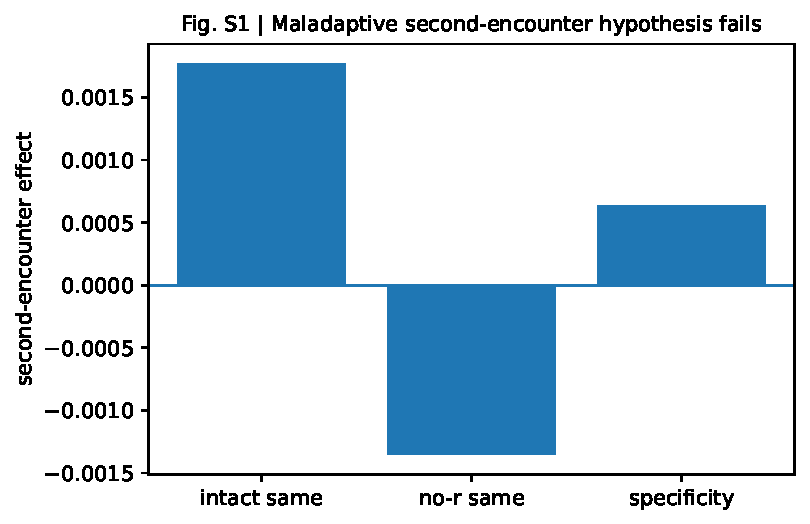
\includegraphics[width=0.82\textwidth]{figures/figS1_maladaptive_null.pdf}
\caption{The maladaptive second-encounter hypothesis fails. The intact same-relation effect is small and positive rather than maladaptive; relevance removal does not produce the planned rescue.}
\end{figure}

\subsection{Collective readout is structured but continuous}

F04 showed that contextual reweighting was not dominated by a single catastrophic discontinuity. The maximum-jump-to-path ratio was approximately $0.0741$ for $b$ and $0.0771$ for action. Curvature increased more strongly around median crossings than around generic rank events; for $b$, the mean median-over-rank curvature advantage was $2.37\times10^{-4}$. Thus the collective median acts as a structured continuous nonlinearity rather than merely as a binary switch.

\begin{figure}[h]
\centering
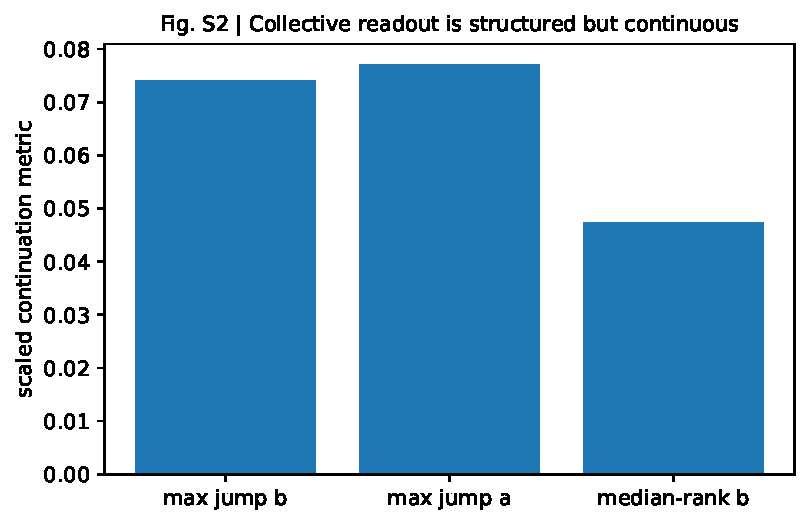
\includegraphics[width=0.82\textwidth]{figures/figS2_continuation.pdf}
\caption{Continuation analysis of collective trace readout. Maximum local jumps remain small relative to full path length; median crossings produce stronger curvature than generic rank events. The median-minus-rank $b$ advantage is multiplied by 200 only for the display scale.}
\end{figure}

\subsection{Both active and slow supports carry turning-point history}

Removing the slow-state family at the turn eliminated mean fraction $0.538682$ of the later response. Within that slow contribution, resetting $m$ alone removed $0.476297$, corresponding to $88.67\%$ of the slow-family effect. Removing fast state accounted for fraction $0.341911$, and resetting $x$ alone removed $0.290799$, corresponding to $84.17\%$ of the fast-family effect. These results motivated the explicit $x\leftrightarrow m$ relay studied later.

\begin{figure}[h]
\centering
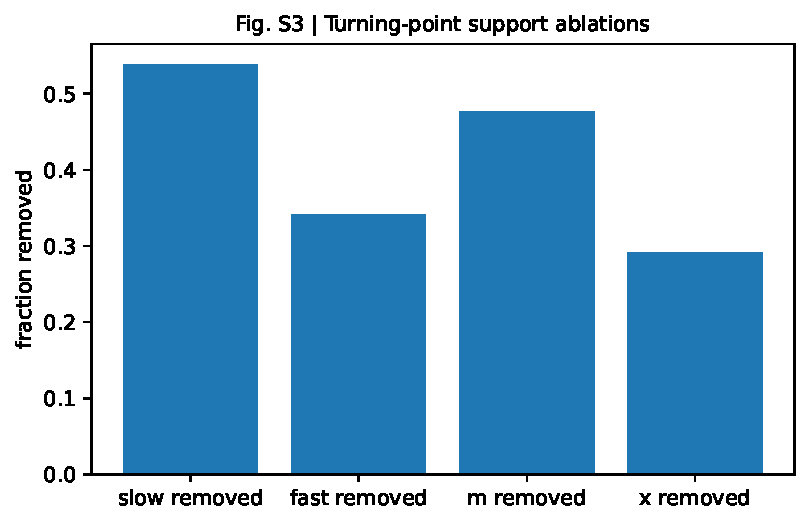
\includegraphics[width=0.82\textwidth]{figures/figS3_turn_ablation.pdf}
\caption{Turning-point support decomposition. Both slow and fast families contribute, with $m$ and $x$ dominating their respective families.}
\end{figure}

\subsection{Partial geometric alignment improves but does not close the relay}

Return alignment increased recurrent-state target projection by $+0.009367$ relative to native and by $+0.012342$ relative to scrambled return. Write-side alignment increased the relevant memory-direction cosine by $+0.184014$ and increased the full-return target projection by $+0.004269$. These improvements established a measurable role for geometry but were far too small to prevent multigenerational extinction.

\begin{figure}[h]
\centering
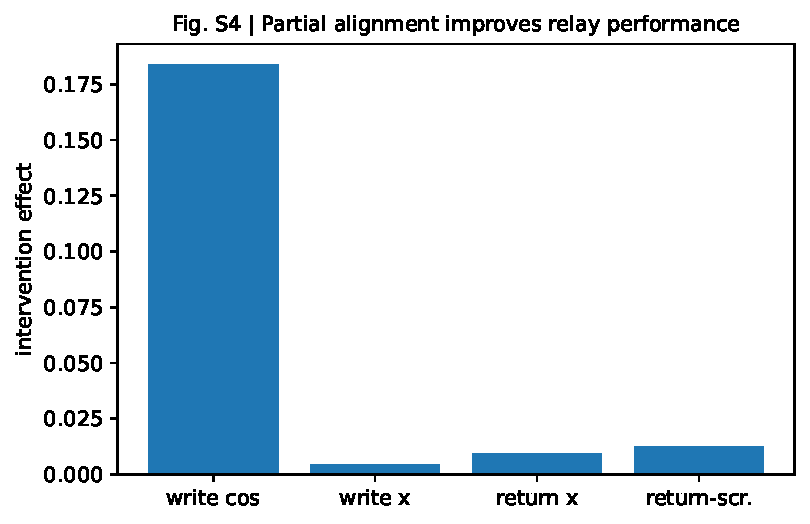
\includegraphics[width=0.82\textwidth]{figures/figS4_partial_alignment.pdf}
\caption{Partial write- and return-side alignment interventions improve relay performance but remain insufficient for repeated recurrence.}
\end{figure}

\subsection{Historical fields do not substantially relocate the dominant loop mode}

Across eight transplanted slow historical packages, the mean pairwise dominant-mode angle was only $0.7953^\circ$, the mean maximum within-seed angle was $1.6135^\circ$, mean projector distance was $0.01963$, and the leading singular-gain spread was $1.13\%$. Historical state can therefore alter downstream operation without substantially relocating the dominant transmission geometry in this protocol.

\begin{figure}[h]
\centering
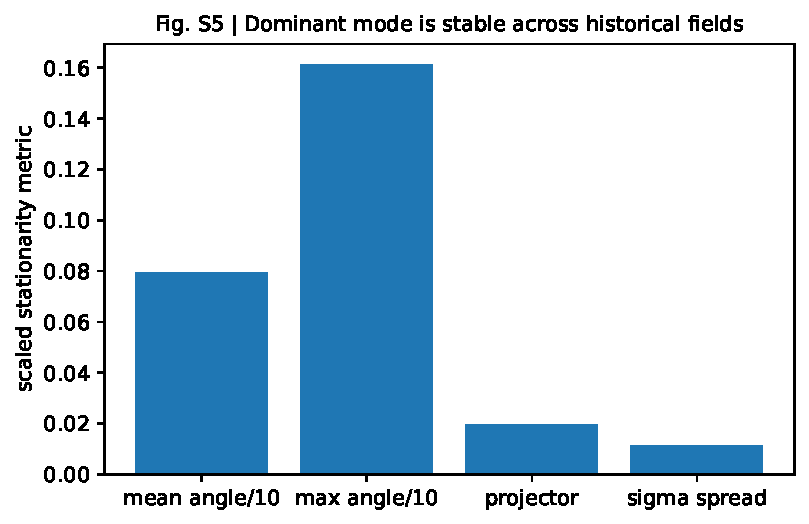
\includegraphics[width=0.82\textwidth]{figures/figS5_history_stationarity.pdf}
\caption{The dominant loop mode is stable across transplanted historical fields. Angle values are divided by ten only for the shared display scale.}
\end{figure}

\subsection{Compatibility is multiplexed in memory amplitude and direction}

In M04, compatibility with the dominant input mode strongly predicted slow-memory imprint magnitude: mean Spearman $\rho=0.926933$, with aligned-to-orthogonal imprint ratio $2.43214$. M05 then separated magnitude and direction. The native relation was $\rho=0.971269$; preserving only the compatibility-dependent imprint amplitude retained $\rho=0.923763$, while preserving only imprint direction retained $\rho=0.862314$. Both channels therefore carry substantial compatibility information.

\begin{figure}[h]
\centering
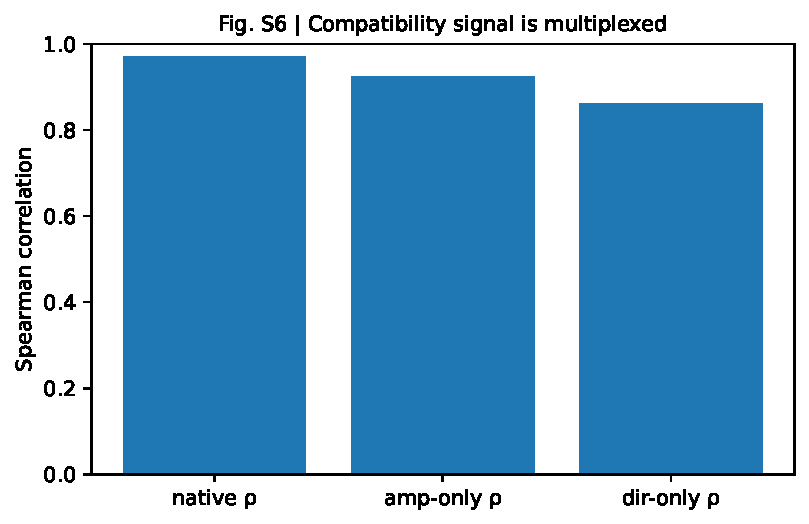
\includegraphics[width=0.82\textwidth]{figures/figS6_compatibility.pdf}
\caption{Compatibility information is multiplexed in slow-memory amplitude and direction.}
\end{figure}

\subsection{Closure is not captured by a common cross-instance map}

The diagnostic C02 common-map analysis yielded held-out mean absolute alignment $0.230768$ for identity, $0.127457$ for common Procrustes, $0.160252$ for ridge regression, and $0.118396$ for the tested state-conditioned reader. No tested common map improved on identity. This diagnostic does not rule out all possible universal nonlinear transformations.

C03 asked a narrower question. A simple within-instance orthogonal bridge reconstructed in calibration context transferred to a distinct context of the same reactor with mean absolute alignment $0.996353$. It beat identity by $0.697708$ and a wrong-instance map by $0.707588$, with all confirmatory seeds favorable. Input and output modal frames were themselves highly stable across contexts ($0.997906$ and $0.998170$ mean alignment). These observations motivated the instance-specific effective causal construction used in C07.

\begin{figure}[h]
\centering
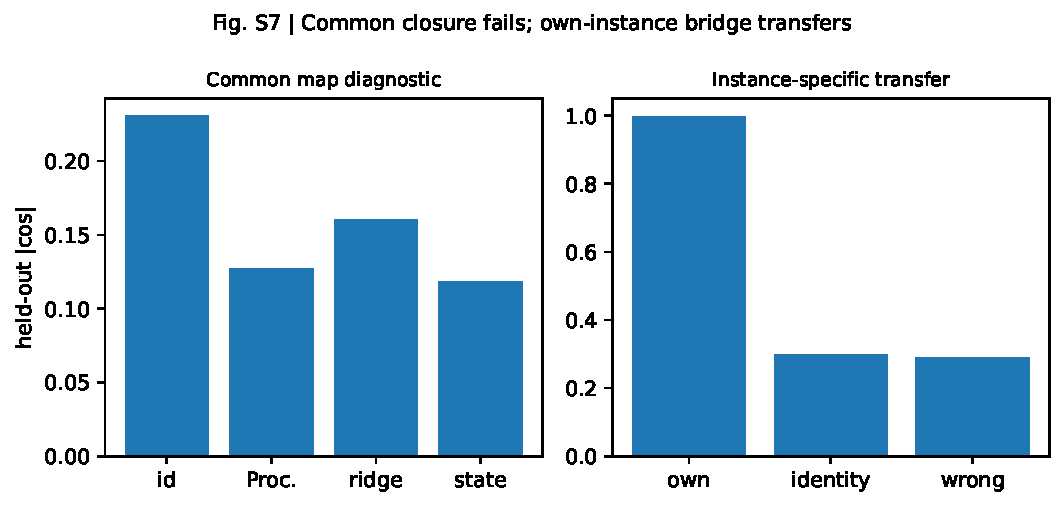
\includegraphics[width=0.95\textwidth]{figures/figS7_common_vs_instance.pdf}
\caption{Common closure maps fail in the tested diagnostic, whereas a simple own-instance bridge transfers across the tested context change.}
\end{figure}

\subsection{Static architectural explanations are insufficient}

C04 tested the simplest reciprocity hypothesis. Exact reciprocity improved one descriptive comparison over native by $+0.18397$, but the stronger frozen reciprocity-specific hypotheses failed: their primary mean advantages were $+0.07051$, $+0.02441$, and $+0.01429$, with favorable-seed fractions $0.6875$, $0.59375$, and $0.546875$. Reciprocity altered behavior but did not robustly supply the predicted closure.

C05 independently manipulated recurrent-state subspace alignment and memory-basis alignment. Recurrent-space matching produced mean effect $+0.10107$ but only $73.44\%$ positive seeds. Memory-basis matching alone produced mean signed effect $-0.01849$. The interaction was $+0.08755$ with only $68.75\%$ favorable seeds, and matching both yielded mean input-output alignment $0.52495$. All frozen primary hypotheses failed. The exploratory C06 moderator analysis also found no useful simple static predictor of heterogeneity; representative correlations were Pearson $r=-0.159$ and Spearman $\rho=-0.107$, while cross-validated ridge models produced negative $R^2$ values ($-0.037$ and $-0.085$).

\begin{figure}[h]
\centering
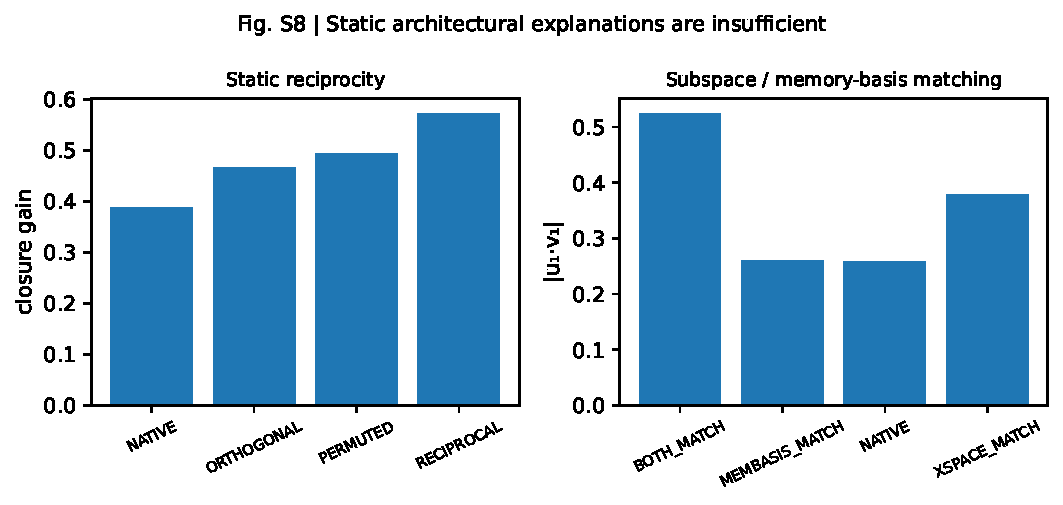
\includegraphics[width=0.95\textwidth]{figures/figS8_static_failures.pdf}
\caption{Static architectural explanations are insufficient. Reciprocity and subspace/basis matching alter the geometry but do not satisfy the stronger frozen closure predictions.}
\end{figure}

\section{Confirmatory criteria for the final repair}

\begin{table}[H]
\caption{Frozen G01 and G02 criteria and observed outcomes.}
\begin{tabular}{p{0.09\textwidth}p{0.41\textwidth}p{0.26\textwidth}c}
Test & Frozen rule & Outcome & Pass\\
\hline
G01 H1 & G4 mean $>0.85$; $>90\%$ seeds $>0.70$; bootstrap lower bound $>0.75$ & mean $0.992131$, fraction $0.96875$, CI $[0.960493,1.021435]$ & yes\\
G01 H2 & correct closure advantage over same-gain/no-closure $>0.70$; $>95\%$ positive; lower bound $>0.60$ & $+0.912540$, all positive, CI $[0.881205,0.941729]$ & yes\\
G01 H3 & advantage over better STATIC/WRONG control $>0.60$; $>90\%$ positive; lower bound $>0.50$ & $+0.792420$, all positive, CI $[0.756705,0.827210]$ & yes\\
G01 H4 & mean G1--G4 postclosure alignment $>0.99$; $>90\%$ seed minima $>0.98$ & mean $0.999136$, fraction $1.0$ & yes\\
G02 H1 & G4 nonorthogonal mean share $>0.95$; $>90\%$ cells $>0.90$; lower bound $>0.93$ & $0.990252$, fraction $0.98958$, CI $[0.987357,0.992740]$ & yes\\
G02 H2 & $67.5^\circ$ increase $>0.70$; $>90\%$ positive; lower bound $>0.65$ & $+0.833120$, all positive, CI $[0.825598,0.839580]$ & yes\\
G02 H3 & FIXED minus same-gain/no-closure $>0.65$; $>95\%$ positive; lower bound $>0.60$ & $+0.873150$, all positive, CI $[0.860523,0.885624]$ & yes\\
G02 H4 & $S_{90^\circ,G1}<0.10$, $S_{67.5^\circ,G1}>0.75$, and $>85\%$ seeds with $S_{67.5}>S_{90}$ & $0.001544$ vs $0.864123$, all seeds ordered & yes\\
\end{tabular}
\end{table}

\section{Reproducibility and provenance}

The public release distinguishes three provenance classes. \texttt{ORIGINAL} denotes artifacts recovered independently from the persistent Library or working archive. \texttt{TRANSCRIPT\_RECOVERED} denotes exact code or design text copied from visible code/JSON blocks in the frozen research transcript. \texttt{REFERENCE\_RECONSTRUCTION} denotes executable replacements reconstructed from the frozen record, recovered designs, original base reactor, downstream APIs, and archived result schemas.

Three transient dependencies fall in the third class: the relational $R_4(\phi)$ scaffold, the full-loop operator scaffold, and the half-channel factorization scaffold. The reconstructed relation passes its prospectively specified causal-signature test across $-135^\circ,-90^\circ,-45^\circ,0^\circ,45^\circ,90^\circ,135^\circ,180^\circ$. The two reconstructed operator scaffolds were audited against archived confirmatory tables. For the eight seed-level validation cases, primary singular-value quantities show correlations approximately $0.98$--$0.999$ with low mean absolute error. Running the reconstructed operators on the full frozen cohorts preserves the primary R06 and R07 confirmatory decisions.

The original transient noise-seed mixer was not independently archived. The reconstruction preserves matched-noise semantics but cannot claim forensic equality of every auxiliary seedwise column. The release therefore claims an executable, source-auditable scientific reproduction pathway, not byte-identical recovery of every transient original file.

Raw research-conversation exports are not distributed in the public repository because they contain unrelated material. Their filenames and SHA-256 hashes are recorded in the provenance manifest, while the scientific design and result artifacts extracted from them are released separately.

\end{document}
